
% !TeX spellcheck = de_DE
\documentclass{article}

\usepackage[ngerman]{babel}
\usepackage{graphicx}
\usepackage{float}
\usepackage{booktabs}
\usepackage{lscape}
\usepackage{longtable}
\usepackage{geometry}
\usepackage{caption}
\usepackage{subcaption}

\graphicspath{ {./images/} }
\setlength\parindent{0pt}

\setlength\LTleft{0pt}
\setlength\LTright{0pt}

\makeatletter
\newcommand{\sectionauthor}[1]{
	{\parindent 0em \large \scshape Autor: #1 \par \nobreak \vspace*{1em}}
	\@afterheading
}
\newcommand{\specification}[3]{
	{\parindent 0.5em \hangindent 3em \hypertarget{spec:#1:#2}{\textbf{/#1#2/}} #3 \par \nobreak \vspace*{0.5em}}
}
\makeatother

\title{BiBi - Implementierungsbericht}
\date{\today\\v1.0}
\author{
	Ivan Charviakou\\
	León Liehr\\
	Jonas Picker\\
	Sergei Pravdin
}

\begin{document}

%--Titel----------------------------------------------------------------------------------------------------------------------------------------------------------------------------------
\maketitle
\begin{figure}[H]
	\centering
	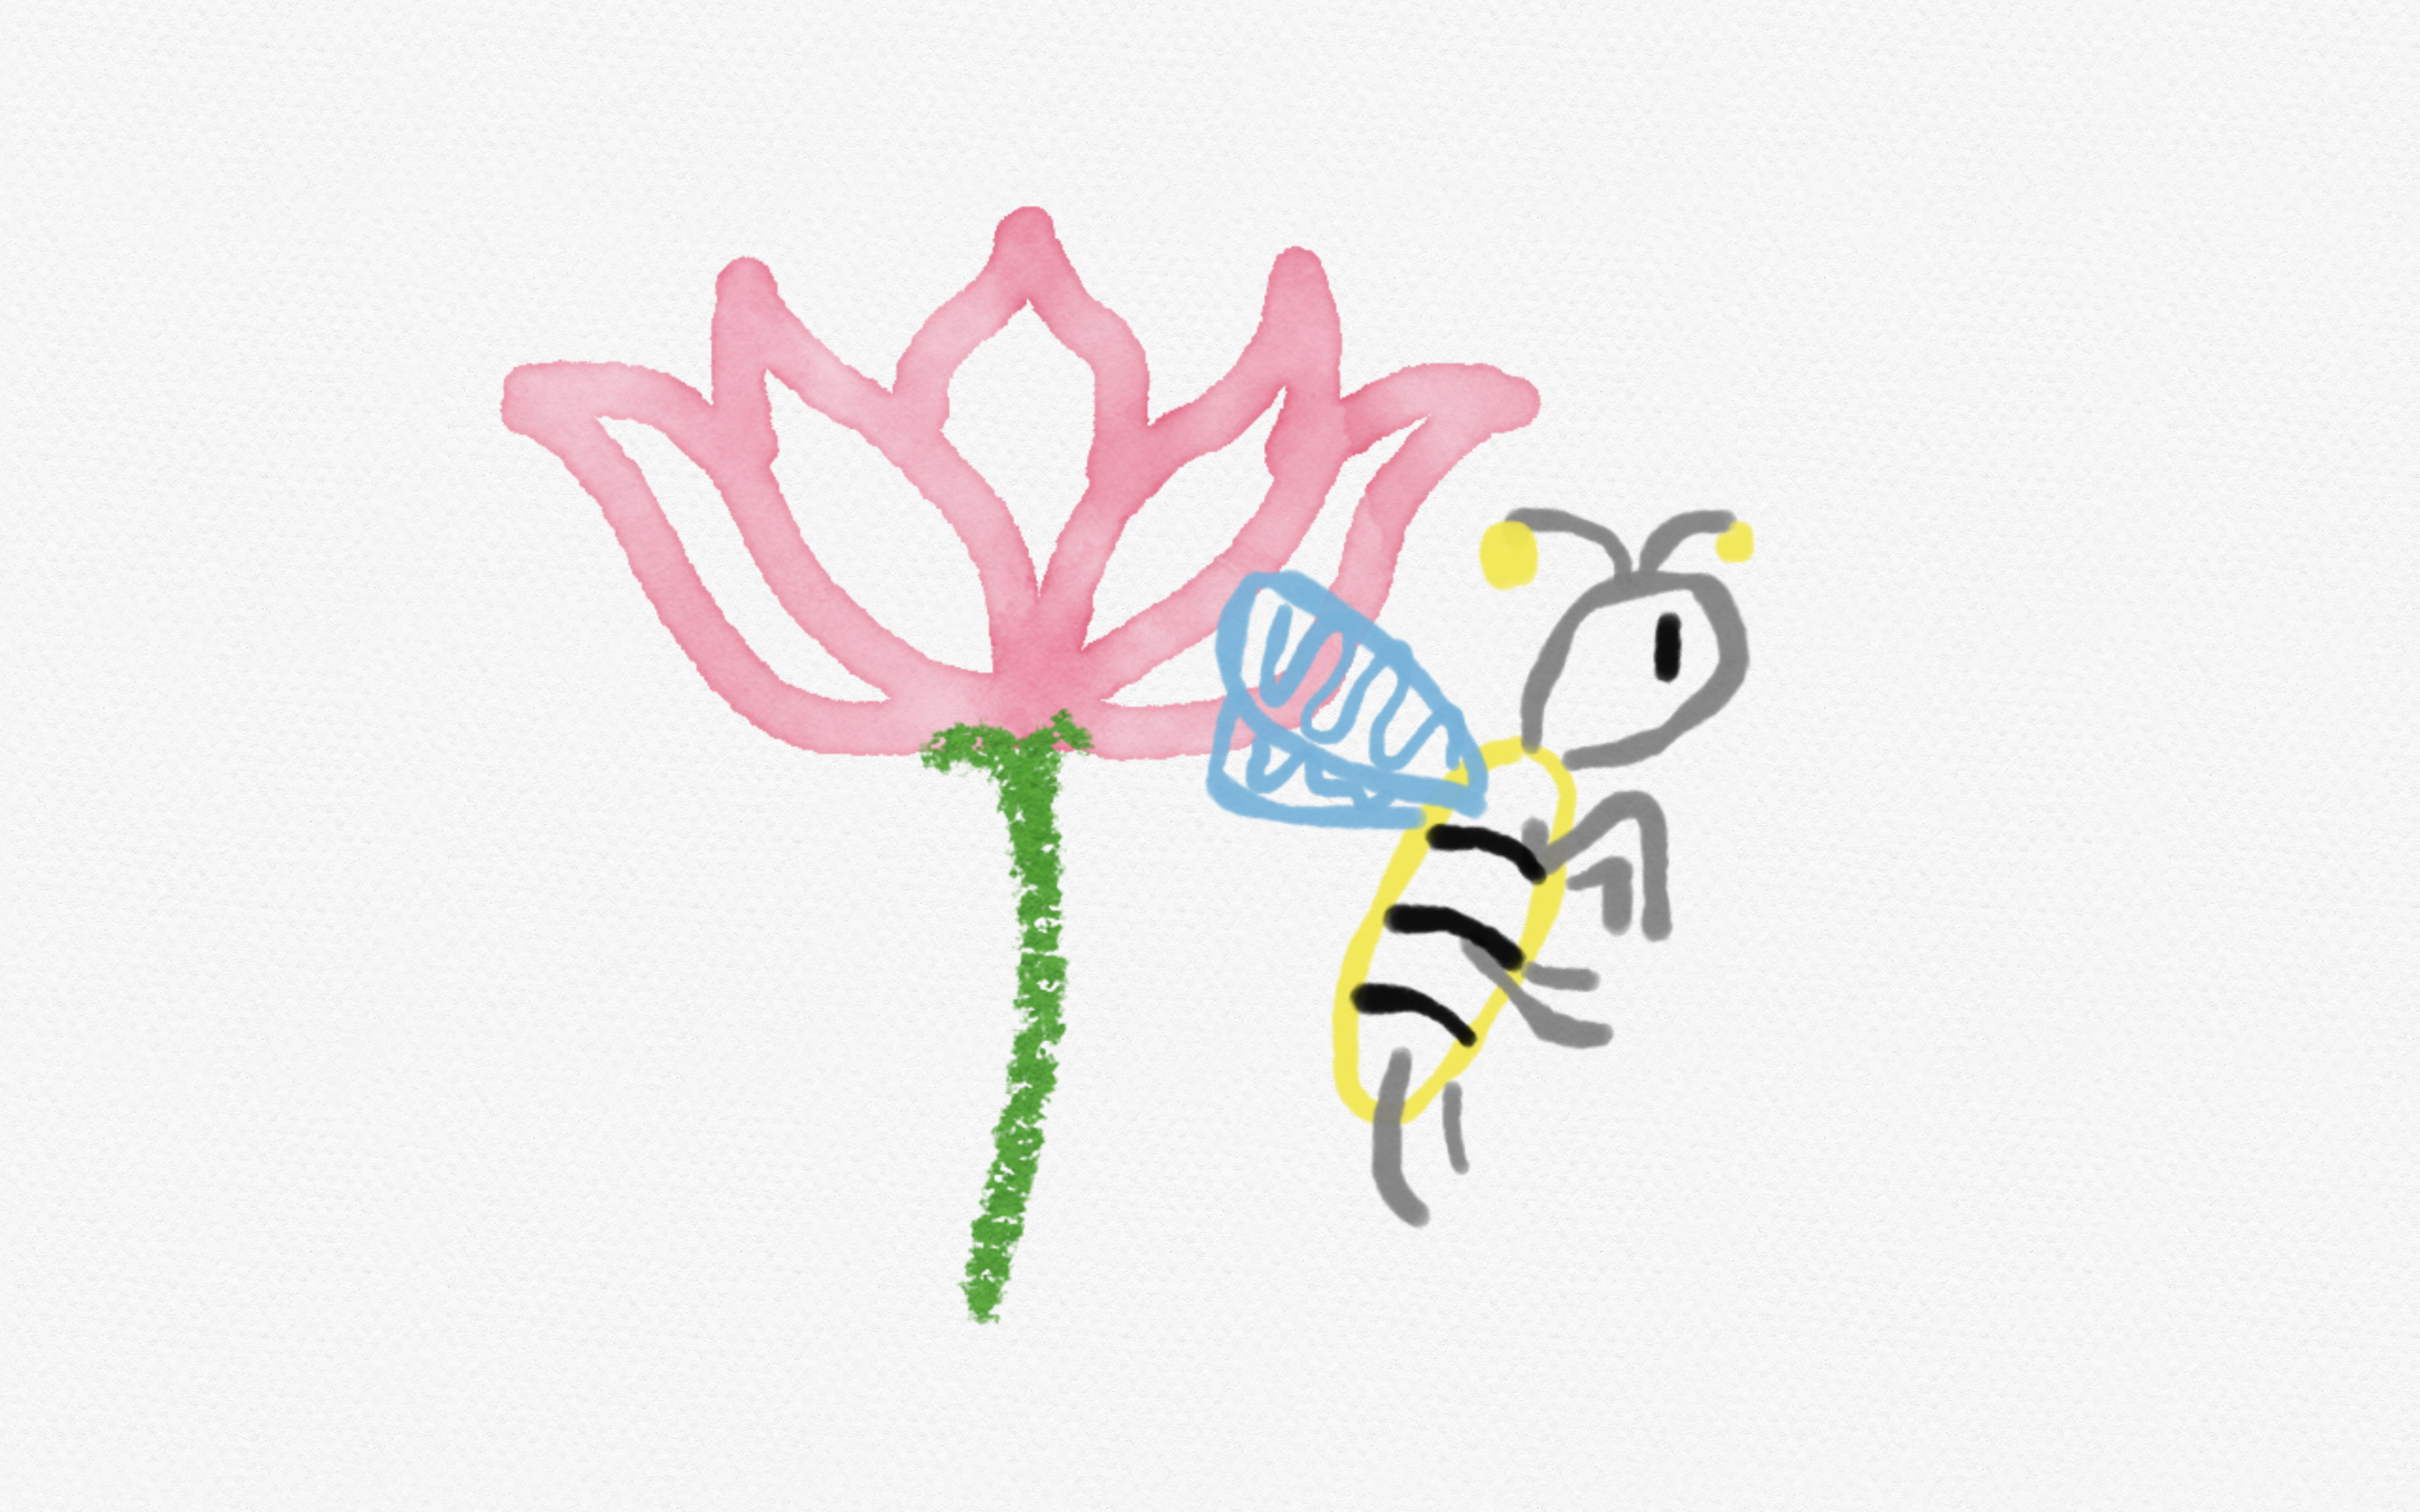
\includegraphics[width = 30em]{Logo}
\end{figure}
\newpage
\tableofcontents
\newpage


\section{Einleitung}%--------------------------------------------------------------------------------------------------
\sectionauthor{Sergei Pravdin}
In diesem Dokument ist der Implementierungsbericht der Webanwendung \textbf{BiBi} dokumentiert. Dabei erfolgt die Gliederung der Implementierung in Milestones mit den geplanten und tatsächlichen Zeitaufwänden. Außerdem sind das \textbf{Änderungen gegenüber der Spezifikation}, die \textbf{Änderungen gegenüber dem Implementierungsplan} und die \textbf{Code-Metriken} zu sehen.

%--Meilensteine----------------------------------------------------------------------------------------------------------------------------------------------------------------------
\section{Meilensteine}
\sectionauthor{Sergei Pravdin}
In diesem Kapitel werden wir die geplanten Zeitaufwänden, bzw. Start- und Endzeiten, mit den tatsächlichen Werten verglichen.

\newgeometry{left=0cm,right=0cm,top=0cm,bottom=2cm}
\begin{figure}[h]
    \centering
    \includegraphics{MS1-2}
    \caption{Meilensteine 1 und 2}
\end{figure}
\restoregeometry

\newpage

\newgeometry{left=0cm,right=0cm,top=0cm,bottom=2cm}
\begin{figure}[h]
    \centering
    \includegraphics{MS3}
\end{figure}
\restoregeometry

\newpage

%--Spezifikation----------------------------------------------------------------------------------------------------------------------------------------------------------------------
\section{Änderungen gegenüber der Spezifikation}
\sectionauthor{León Liehr}

\begin{itemize}
    \item Mehrere Typen wie \texttt{UserRole}, \texttt{SearchOperator}, \texttt{UserLendStatus} wurden von dem Paket \texttt{model.logic.util} in das Paket \texttt{model.data} verschoben, welches die DTOs enthält, da diese ausschließlich schlichte Daten darstellen (d.h. keine Programmlogik mit sich tragen).
    \item Die zuvor in JSFs EL verfassten Ausdrücke, welche die Sichtbarkeiten von Bedienelementen auf verschiedenen Facelets wie der Kopfzeile regelten, wurden größtenteils in eigenständige Java-Methoden der jeweiligen Backing Bean umgeschrieben, um die Anwendungslogik weiter von der View zu trennen. Die Namen jener Methoden beginnen konventionell mit \texttt{isShowing}.
    \item Es wurde eine Methode \texttt{isStaffOrHigher} unter der Klasse \texttt{UserRole} erstellt, welche in mehreren BBs verwenden wird, sodass der Code nicht dupliziert werden muss.
    \item Die Methoden \texttt{getAllSearchOperators} und \texttt{getAllSearchCriteria} wurde für das BB\\ \texttt{UserSearch} kreiert. Diese delegieren an die entsprechende statische \texttt{values}-Methode der korrespondierenden Aufzählung, die sonst aus technischen Gründen nicht in der EL referenzierbar ist. Sie füllen die \texttt{<h:selectOneMenu>}s mit Daten via \texttt{<f:selectItems>}.
    \item Es wurde die statische Methode \texttt{readCopiesReadyForPickupAllUsers} in \texttt{MediumDao} definiert, welche unabdingbar für das BB \texttt{copies-ready-for-pickup-all-users} ist, leider aber in der Spezifikation vergessen wurde.
    \item Das Paket \texttt{backingbeans} wurde in \texttt{backing\_beans} umbenannt, um der Namenskonvention von Paketen zu folgen.
    \item Die BB \texttt{DirectLending} wurde in \texttt{Lending} umbenannt und das Facelet \texttt{direct-lending} in \texttt{lending}, weil das eliminierte Präfix nicht zu Verständnis beitrug und inkonsistent mit \texttt{ReturnForm} war.
    \item Das Konzept von dynamischen Medienattributen wurde ersetzt durch einen festen Satz, welcher als Datenbankspalten umgesetzt wurde und neben anderen die Attribute \textit{Titel}, \textit{Verlag} und \textit{Erscheinungsjahr} enthält. Daraus resultierend wurden jegliche assoziierten Klassen und DAO-Methoden entfernt.
    Dazu zählen die DTOs \texttt{AttributeDto}, \texttt{AttributeType}, die Typen \texttt{AttributeMultiplicity} und \texttt{MediumPreviewPosition}. Des Weiteren wurde der Mediumschema-Editor obsolet und wurde gelöscht. Die Klasse \texttt{AttributeOrCategory} wurde in eine Aufzählung \texttt{MediumSearchCriterion} abgewandelt, welche den nun festen Attributsatz einbindet. Zusammenfassend gesagt durchlebten mehrere Facelets und BBs wie die Mediensuche und die Medienansicht kleinere Anpassungen, um diese neue Struktur verwenden zu können.
    Diese Änderungen sind in der allgemeinen Reduktion des Arbeitsumfangs dieses Teams begründet, die ihrerseits auf dem Ausschluss des Gruppenmitglieds Mohamad Najjars basiert.
    \item Zusammenhängend mit dem Obigen gibt es jetzt keine mehrwertigen Medienattribute von willkürlicher Länge mehr. Das einzige übriggebliebene einst $n$-stellige Attribut \textit{Autoren} des Beispielattributsatzes wurde in die fünf Attribute \texttt{author1}, \textellipsis, \texttt{author5} aufgelöst. Die Motivation ist identisch.
    \item Medienattribute können nun nur noch Text sein und kein Hyperlink oder Bild. Ferner kann kein Logo mehr über die Verwaltungsseite hochgeladen werden. Diese Entscheidung geht aus der allgemeinen Arbeitsumfangsverringerung hervor. Das Datenbankschema wurde entsprechend angepasst.
    \item Es wurden mehrere Validatoren und Konverter hinzugefügt, die in der Spezifikation übersehen wurden. Dazu zählen \texttt{LendingProcessSignatureValidator}, \texttt{ReturnFormSignatureValidator} und \texttt{MediumCreationSignatureValidator}.
    \item Neue Exceptions wurden geschaffen inklusive \texttt{CategoryDoesNotExistException} und\\ \texttt{UserExceededDeadlineException}. Diese erlauben präzisere Fehlerbehandlung und Berichterstattung.
    \item Ein Vielzahl an Umbenennungen fand aufgrund einer Verbesserung des Leseverständnisses statt. Dazu zählt \texttt{UserSearchDto\#userLendStatus} (\textrightarrow{} \texttt{UserSearchDto\#lendStatus}), \texttt{MediumSearch\#searchMedium} (\textrightarrow{} \texttt{MediumSearch\#searchMedia}), \texttt{UserSearch\#searchUser} (\textrightarrow{} \texttt{UserSearch\#searchUsers}), \texttt{UserDao.readUserBySearchCriteria} (\textrightarrow{} \texttt{searchUsers}).
    \item Eine Utility-Klasse \texttt{Pagination} wurde definiert, um Logik zu kapseln, die in mehreren DAO-Methoden vorkommt, die mit paginierten Listen arbeiten.
    \item Die Seite für Leihfristverstöße ist nun auch zugänglich für Bibliotheksmitarbeiter und nicht nur für Administratoren. Erstere ziehen einen viel größeren Nutzen aus dessen Erreichbarkeit als letztere.
    \item Mehr Hyperlinks wurden der Kopfzeile (dem Header) hinzugefügt wie welche zu der Nutzersuche, zu den Leihfristverstößen und zu dem Kategorienstöberer. Davor wurde mit der Einführung von Drop-Down-Menüs Platz geschaffen.
    \item Die Komponente \texttt{<bibi:reactiveInputField>} wurde überall durch \texttt{<h:inputText>} ersetzt und überhaupt nicht implementiert, um den allgemeinen Arbeitsumfang des Teams zu verkleinern.
    \item Die abstrakte Klasse \texttt{PaginatedList}, das DTO \texttt{PaginationDto} und das Composite Component \texttt{paginatedList} wurde überarbeitet. Die Spezifikation stellte sich als löchrig heraus.
    \item Der Ordner \texttt{view/public} wurde in \texttt{view/ffa} und \texttt{view/opac} aufgespalten, um die Idee der Öffnung und Schließung des Systems erweiterbar (i.e. ohne hartkodierte Liste von Dateipfaden) umsetzen zu können.
\end{itemize}

%--Implementierungsplan----------------------------------------------------------------------------------------------------------------------------------------------------------
\section{Änderungen gegenüber dem Implementierungsplan}
\sectionauthor{Jonas Picker}
Im Folgenden werden die Abweichungen vom Implementierungsplan
\subsection{Milestone 1}
Zu Beginn des Milestones am Montag den 31.05.2021 war es zunächst notwendig, den bisherigen Implementierungsplan aufgrund von Unzulänglichkeiten komplett zu überarbeiten. Im Zuge dessen wurde der eigentliche Beginn der Implementierungsarbeit für 3 Teammitglieder deutlich verzögert. Das restliche Kapitel bezieht sich auf diese zweite, überarbeitete Version des Plans. Es war ursprünglich geplant, den Testspezialisten das Schreiben der Testpakete übernehmen zu lassen und ihn zum Ausgleich in den anderen Paketen zu entlasten. Nachdem dies wider Erwarten nicht stattfinden konnte, mussten alle Teammitglieder zusätzliche Zeit aufwenden, um sich teilweise parallel in das verwendete Testframework einzuarbeiten. Das Aufsetzen der Datenbank und der Systemstartfunktionen nahm ebenfalls deutlich mehr Zeit in Anspruch, als ursprünglich angenommen. Nachdem sich dieses Arbeitspaket (`SystemStartStop/DataLayerInitializer') auch als schwierig zu testen herausstellte, wurde der geplante Test stattdessen zunächst für den Logger erstellt. Durch die Entscheidung, die Tests nicht mit Auszuliefern und in ein eigenes Projekt zu verpacken, entstanden hier bereits die ersten Probleme beim Lesen von Dateien aus dem Hauptprojekt, jedoch wurde es aus Zeitmangel und der unerwarteten Parallelarbeit an den Tests nicht gleich kollektiv erkannt. Durch falsch kalkulierte Zeitschätzungen beim Anpassen des Implementierungsplans am Anfang der Phase, hatte der Testspezialist zum Schluss zu wenig Arbeit und es wurde bereits mit Teilen des Arbeitspakets `Medienansicht' aus Milestone 2 begonnen. Neben Problemen bei der korrekten Fertigstellung des Arbeitspakets `Login/Registrierung', hatte der verantwortliche Implementierer Schwierigkeiten, das Versionskontrollsystem `git' im Einklang mit dem übrigen Team und dem Spezialisten über die Kommandozeile zu benutzen. Dadurch entstand ein deutlicher Mehraufwand für den Rest des Teams beim Reparieren unbedachter Operationen am gemeinsamen Repository.

\subsection{Milestone 2}
Wegen des Fehlens eines funktionierenden Logins am Ende von Milestone 1, musste der Verantwortliche dessen Fertigstellung zunächst vervollständigen, wodurch seine geplanten Arbeitspakete in diesem Milestone nicht angefangen wurden. Durch dieses Fehlen einer Grundfunktionalität, wurde das manuelle Ausprobieren von sessionabhängigen Funktionen ebenfalls erschwert. Ansonsten konnten die übrigen Teammitglieder ihre Pakete des zweiten Milestones relativ unabhängig voneinander implementieren, da die Arbeitspakete im Gegensatz zu Milestone 1 horizontal aufgebaut waren. Am Donnerstag den 10.06.2021 verließ der nacharbeitende Implementierer das Team, ohne eines seiner bisherigen Arbeitspakete vervollständigt zu haben. Dies hatte sowohl eine Reduzierung des Funktionsumfangs des Systems, als auch ein erneutes Umstrukturieren des Implementierungsplans zur Folge, um die fehlende Arbeitskraft zu kompensieren und wichtige Kernfunktionalitäten auf die übrigen Entwickler zu verteilen. Hierbei entstand ein zu großer Mehraufwand für einen unserer Entwickler, der bereits Zeitprobleme hatte und so ebenfalls seine Arbeitspakete zum Ende von Milestone 2 nicht komplett fertigstellen konnte. Im Testprojekt kristallisierte sich gegen Ende des Milestones heraus, dass der Pfad zur Konfigurationsdatei aus dem Hauptprojekt trotz mehrstündiger Versuche nicht aufgelöst werden konnte und deshalb der ConnectionPool keine Verbindung zur Datenbank bekam. Die Lösung dieser Schwierigkeit wurde aus Zeitmangel in den letzten Milestone verschoben.

\subsection{Milestone 3}
Neben der Nacharbeit der fehlenden Pakete aus dem letzten Abschnitt, war es dem Entwickler diesmal möglich, auch seine übrigen Arbeitsaufträge zu erfüllen. Hierzu wurden nicht nennenswerte Teile von Arbeitspaketen als kleine Entlastung umverteilt. Das Leseproblem im Testprojekt wurde umgangen, indem im PreTest die Konfigurationsdatei hartkodiert übergeben wurde. Ohne eine explizite Lösung des Problems war jedoch ein Fertigstellen des im Abschnitt 1 erwähnten Loggertests nicht möglich, dieser wurde gestrichen und gegen einen Test für den DataLayerInitializer ausgetauscht. Außerdem wurde die Reihenfolge der Pakete verändert, z.B. wurde die Implementierung des TrespassListeners nach hinten verlegt, um manuelle URL-Eingaben für unkompliziertes Testen bis zum Ende des Milestones möglich zu machen. Es trat dann Mitte der Woche eine bis jetzt ungeklärte Anomalie bei zwei unserer Entwickler auf, in Folge derer sich das System lokal nicht mehr starten lies. Da unser Paginationsspezialist, der das Gros der verbleibenden technisch komplizierten Teile nach der Funktionsreduktion zu tragen hatte, so noch zusätzlich Zeit aufwenden musste, geriet er mit den Tests in Verzug und es wurde beschlossen, diese zeitnah nachzuliefern. Ohne die Möglichkeit, produzierten Code zu testen, verschob sich ebenfalls die Fertigstellung des Kategoriebrowsers über das Ende des Milestones hinaus.

\subsection{Allgemeine Schwierigkeiten}
Eigene Implementierungen der nötigen Validatoren und Converter für das reibungslose Funktionieren der Facelets wurden in vorhergehenden Phasen großteils gar nicht spezifiziert und stellten einen ungeplanten Mehraufwand in vielen Paketen dar. Ebenfalls ungenügend und zeitaufwendig waren die Kommentare und Methodenrümpfe aus der Spezifikation, die beim Erreichen des Arbeitspakets dann angepasst werden mussten, obwohl diese bereits manchmal als Schnittstelle in anderen Paketen benutzt wurden. Da die Verantwortlichkeiten in den Dao-Klassen methodenweise verteilt waren, kam es teils vor, dass identische Hilfsmethoden redundant parallel entwickelt wurden oder im umgekehrten Fall, Hilfsmethoden von anderen verwendet und dann vom Originalautor abgeändert wurden. Durch die Reduzierung der Teamgröße und damit des Funktionsumfangs mitten in der Implementierungsphase, entstanden einige unbenutze Artefakte im Code und der Datenbank, deren Entfernung weitreichende Änderungen in den Zuständigkeitsbereichen unterschiedlicher Entwickler zur Folge gehabt hätten. Da dies oft nicht mit dem jeweiligen Zeitplan vereinbar war, wurde von deren Entfernung zunächst abgesehen. Infolgedessen rutschten Fertigstellungen von Paketen gegen Ende der Milestones oft in Zeitknappheit und aus Prioritätsgründen wurde dann die Lauffähigkeit und der Umfang der geplanten Testfälle vernachlässigt. Über alle Milestones hinweg gab es immer wieder verschiedene Probleme, die mit der Interaktion unseres Versionskontrollsystems und den unterschiedlichen Entwicklungsumgebungen der Teammitglieder zusammenhing. Hierbei wurden vor allem Projektkonfigurationen die in proprietären Metadatenformaten der jeweiligen IDEs gespeichert waren, immer wieder gegenseitig überschrieben und es gab Unterschiede in der Interpretierung der Packagestruktur. All dies resultierte in der Notwendigkeit für einige Mitglieder, mitten in der Implementierungsphase auf die Referenzentwicklungsumgebung zu wechseln, womit weitere ungeplante Einarbeitungszeit einherging.

%--Metriken----------------------------------------------------------------------------------------------------------------------------------------------------------------------------
\section{Code-Metriken}
\sectionauthor{Ivan Charviakou}

Im Folgenden werden verschiedene Code-Metriken allgemein vorgestellt und für das erstellte Projekt angegeben.
Darüber hinaus lassen sich diese Metriken in drei allgemeine Untersuchungsbereiche unterteilen:
Allgemeine Metriken, Komplexitäts-bezogene Metriken, und Abhängigkeits-bezogene Metriken.
Durch Angabe dieser Metriken wird eine genauere Analyse des Codes aus verschiedenen Sichten ermöglicht.

\subsection{Allgemeine Metriken}

%--Table for facelets
\begin{longtable}{@{\extracolsep{\fill}}lcl@{}}
\toprule
\multicolumn{2}{l}{\textbf{Facelets}} \\* \midrule
\endfirsthead
\endhead
\textbf{Anzahl Facelets} & 29 \\
\textbf{Anzahl Zeilen XML Code} & 1664 \\* \bottomrule
\end{longtable}

%--Table for packages
\begin{longtable}{@{\extracolsep{\fill}}lclclcl@{}}
\toprule
\multicolumn{4}{l}{\textbf{Metriken nach Paket}} \\* \midrule
\textbf{Paketname} & \textbf{\begin{tabular}[c]{@{}l@{}}Anzahl\\ Java-Zeilen\end{tabular}} & \textbf{\begin{tabular}[c]{@{}l@{}}Anzahl\\ Java-Methoden\end{tabular}} & \textbf{\begin{tabular}[c]{@{}l@{}}Anzahl\\ Java-Klassen\end{tabular}} \\* \midrule
\endfirsthead
\textbf{Paketname} & \textbf{\begin{tabular}[c]{@{}l@{}}Anzahl\\ Java-Zeilen\end{tabular}} & \textbf{\begin{tabular}[c]{@{}l@{}}Anzahl\\ Java-Methoden\end{tabular}} & \textbf{\begin{tabular}[c]{@{}l@{}}Anzahl\\ Java-Klassen\end{tabular}} \\* \midrule
\endhead
...data.dtos 				& 852 		& 200 		& 23 \\
...data.exceptions			& 4 			& 1	 		& 1 \\
...model.logic.converters			& 218 		& 14	 		& 10 \\
...model.logic.exceptions			& 183 		& 25	 		& 6 \\
...model.logic.managed\_beans		& 2203		& 240 		& 27 \\
...model.logic.util					& 369		& 23			& 14 \\
...model.logic.validators			& 443 		& 16	 		& 11 \\
...model.persistence.daos			& 2518 		& 111 		& 4 \\
...model.persistence.exceptions		& 407 		& 76	 		& 19 \\
...model.persistence.util			& 950 		& 51	 		& 10 \\
Insgesamt	 							& 8147 		& 757 		& 125 \\* \bottomrule
\end{longtable}

\subsection{Komplexitäts-bezogene Metriken}

%--Table for packages
\begin{longtable}{@{\extracolsep{\fill}}lclclcl@{}}
\toprule
\multicolumn{4}{l}{\textbf{Metriken nach Paket}} \\* \midrule
\textbf{Paketname} & \textbf{Durchschnittliche zyklomatische Komplexität*} \\* \midrule
\endfirsthead
\textbf{Paketname} & \textbf{Durchschnittliche zyklomatische Komplexität} \\* \midrule
\endhead
...model.data.dtos 				& 1.14 \\
...model.logic.converters			& 1.64 \\
...model.logic.exceptions			& 1.24 \\
...model.logic.managed\_beans		& 1.44 \\
...model.logic.util					& 2.48 \\
...model.logic.validators			& 3.06 \\
...model.persistence.daos			& 2.88 \\
...model.persistence.exceptions		& 1 \\
...model.persistence.util			& 2.14 \\* \bottomrule
\end{longtable}

%--Table for methods
\begin{longtable}{@{\extracolsep{\fill}}lcl@{}}
\toprule
\multicolumn{2}{l}{\textbf{Die 10 komplexeste Methoden nach kognitiver Komplexität}} \\* \midrule
\textbf{Methodenname} & \textbf{Kognitive Komplexität*} \\* \midrule
\endfirsthead
\textbf{Methodenname} & \textbf{Kognitive Komplexität} \\* \midrule
\endhead
\begin{tabular}[c]{@{}l@{}}de.dedede.model.persistence.util.\\DataLayerInitializer.consoleDialogue(Connection)\end{tabular}									& 21 \\
\begin{tabular}[c]{@{}l@{}}de.dedede.model.persistence.util.\\DataLayerInitializer.setUpDatabase()\end{tabular} 											& 20 \\
\begin{tabular}[c]{@{}l@{}}de.dedede.model.logic.managed\_beans.\\Lending.lendCopies()\end{tabular}													& 18 \\
\begin{tabular}[c]{@{}l@{}}de.dedede.model.logic.util.\\TrespassListener.afterPhase(PhaseEvent)\end{tabular}												& 18 \\
\begin{tabular}[c]{@{}l@{}}de.dedede.model.logic.managed\_beans.\\ReturnForm.returnCopies()\end{tabular}												& 15 \\
\begin{tabular}[c]{@{}l@{}}de.dedede.model.persistence.daos.\\CategoryDao.createCategory(CategoryDto)\end{tabular}										& 14 \\
\begin{tabular}[c]{@{}l@{}}de.dedede.model.persistence.daos.\\MediumDao.getAppliedLendingLimit(Connection,String,int)\end{tabular}							& 14 \\
\begin{tabular}[c]{@{}l@{}}de.dedede.model.persistence.util.\\MaintenanceProcess.MaintenanceThread.run()\end{tabular}									& 12 \\
\begin{tabular}[c]{@{}l@{}}de.dedede.model.persistence.daos.\\MediumDao.translateNuancedSearchQuery\\(StringBuilder,List,NuancedSearchQuery)\end{tabular}		& 11 \\
\begin{tabular}[c]{@{}l@{}}de.dedede.model.logic.managed\_beans.\\CategoryCreator.onload()\end{tabular}												& 10 \\* \bottomrule
\end{longtable}

\paragraph{Zyklomatische Komplexität}
Als zyklomatische Komplexität bezeichnet man die maximale Anzahl an Pfaden im entsprechenden Kontroll-Fluss Grahpen, die sich jeweils im Vergleich zu allen anderen Pfaden in der Menge an besuchten Knoten um mindestens einen unterscheiden.

\paragraph{Kognitive Komplexität}
Im Code setzt sich die Metrik zur kognitiven Komplexität aus der Anzahl an Brüchen im Kontrollfluss und Verschachtelungen von entsprechenden Kontrollflussanweisungen zusammen.
Im Gegensatz zur zyklomatischen Komplexität fasst diese Metrik die Schwierigkeit, mit der das gegebene Code zum Lesen und Verstehen ist.

\subsection{Abhängigkeits-bezogene Metriken}

%--Table for packages
\begin{longtable}{@{\extracolsep{\fill}}lclcl@{}}
\toprule
\multicolumn{3}{l}{\textbf{Metriken nach Paket}} \\* \midrule
\textbf{Paketname} & \textbf{\begin{tabular}[c]{@{}l@{}}Anzahl\\ Paket-\\Abhängigkeiten\end{tabular}} & \textbf{\begin{tabular}[c]{@{}l@{}}Anzahl Paketen\\ mit dieser\\ Abhängigkeit\end{tabular}} \\* \midrule
\endfirsthead
\textbf{Paketname} & \textbf{\begin{tabular}[c]{@{}l@{}}Anzahl\\ Paket-\\Abhängigkeiten\end{tabular}} & \textbf{\begin{tabular}[c]{@{}l@{}}Anzahl Paketen\\ mit dieser\\ Abhängigkeit\end{tabular}} \\* \midrule
\endhead
de.dedede.model.data.dtos				& 1		& 8 \\
de.dedede.model.data.exceptions			& 0		& 2 \\
de.dedede.model.logic.converters			& 2		& 0 \\
de.dedede.model.logic.exceptions			& 2		& 1 \\
de.dedede.model.logic.i18n				& 0		& 0 \\
de.dedede.model.logic.managed\_beans		& 6		& 2 \\
de.dedede.model.logic.util					& 4		& 6 \\
de.dedede.model.logic.validators			& 4		& 0 \\
de.dedede.model.persistence.daos			& 4		& 4 \\
de.dedede.model.persistence.exceptions		& 1		& 6 \\
de.dedede.model.persistence.util			& 4		& 4 \\* \bottomrule
\end{longtable}


\end{document}


